\section{Implementation}
Game Mechanics function as basic systems of a game that governs their respective game elements (\cite{adams2012game}). All possible basic functions(represented by algorithms and data structures) and rules in the game are part of the mechanics. The section will discuss about planned game mechanics and the project's implementation.

\subsection{Web application}
The game will be a web application, this is because web applications are easily accessible and can be played on any device with a web browser. The game will be built using Angular as its frontend, a popular web application frontend framework and Flask as its backend, as it is a python lightweight backend compared to its alternatives. The UI was developed with PixiJS, A HTML5 creation engine that renders 2D graphics. There was no generic game engine used.

As central storing database, MongoDB was used. This is because MongoDB is a NoSQL database, which is a good choice for storing JSON data and long strings of user code. This database's main purpose is to stores all relevant information regarding the game content and will contain possible analytics in the future. It's base entity is the "Users" entity as shown in Figure \ref{fig:users}.
\begin{figure}[h]
    \centering
    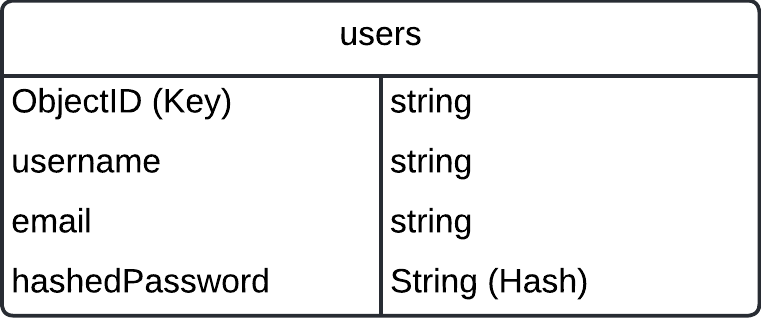
\includegraphics[width=0.5\linewidth]{images/user_object.png}
    \caption{Database model of the \textit{Users} entity}    
    \label{fig:users}
\end{figure}

\subsection{Level selection}
The game will have multiple levels, each level will have a different set of challenges. The player will have to complete each level to progress to the next. The levels will be designed to increase in difficulty as to teach the player different concepts of Python programming.

In the initial level selection, the player will be presented with a list of levels. Each level will have a title, a description, and a button to start the level. The player will be able to see the buttons of the levels they cannot access disabled and greyed out until they have completed the previous level. This is kept track by the leaderboard, which will be discussed in the next section.

\subsection{Leaderboard}
The game will have a leaderboard that will keep track of the player's progress. The leaderboard will store each player's data in the form of an entity in the database as shown in Figure \ref{}. The leaderboard will be updated in real-time as the player progresses through the game. The leaderboard will be stored in the database and will be accessible to all players.
\begin{figure}[h]
    \centering
    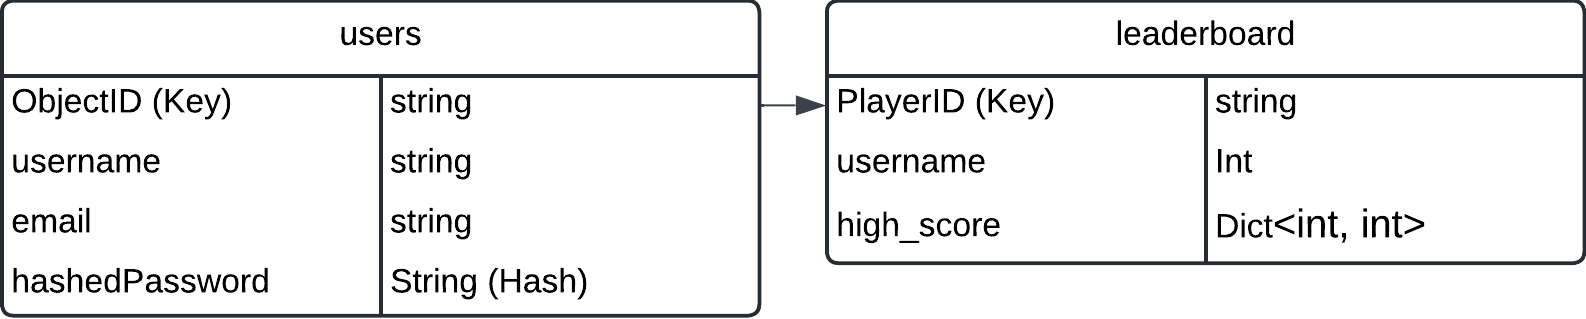
\includegraphics[width=0.5\linewidth]{images/leaderboard_object.png}
    \caption{Database model of the \textit{Leaderboard} entity}    
    \label{fig:users}
\end{figure}
The backend will have an endpoint to handle the leaderboard, this endpoint will have basic CRUD functionality. It will also handle data validation and edge cases in a following manner:
\begin{itemize}
    \item \textbf{Create:} The endpoint will create a new entry in the leaderboard if the player does not have an entry already. This will be done when a player completes a level for the first time. 
    \item \textbf{Read:} The endpoint will read the leaderboard, this will be done when a player wants to view the leaderboard.
    \item \textbf{Update:} The endpoint will update the leaderboard, this will be done when a player completes a level.
    \item \textbf{Delete:} The endpoint will delete an entry in the leaderboard, this will be done when a player wants to remove their entry from the leaderboard.
\end{itemize}

\subsection{Code Input}
The whole user flow of the educational game, game flow\cite{kramarzewski2018practical}, can be simplified. It starts out with the user input, which would be the code submitted, the process would be the gameplay mechanics and the output would be the reward for the player. 

This whole user experience starts with the user input, the submission of code can be done with a simple basic text box.
\begin{figure}[h]
    \centering
    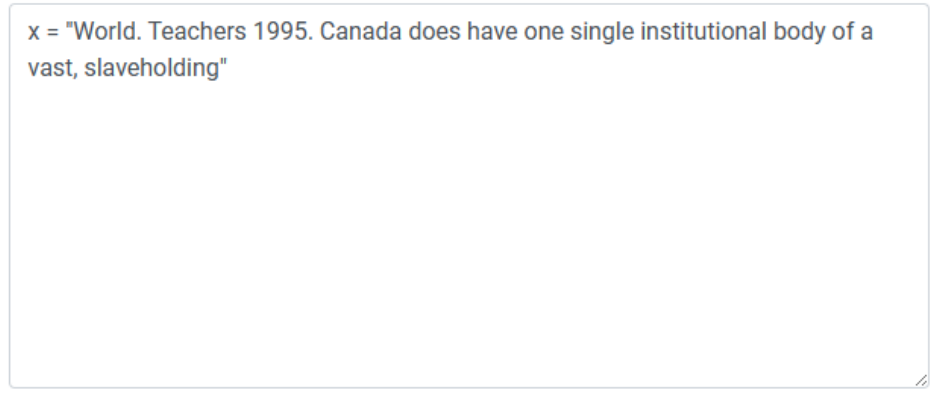
\includegraphics[width=0.5\linewidth]{images/textbox.png}
    \caption{Simple basic text box}
\end{figure}
\\\\
To improve on this submission of code, we can use a code editor like professional integrated development environments (IDEs). An in-browser code editor such as Monaco or ace editor would suffice; additional improvements to build upon a code editor with other options such as night/day mode, a language server to verify Python syntax formatting, and other such Python language features as it is not natively implemented within editors such as Monaco. Other features that should be implemented to help with user experience would be code completion, syntax/semantic highlighter, definition provider, formatting provider, and more.
\begin{figure}[H]
    \centering
    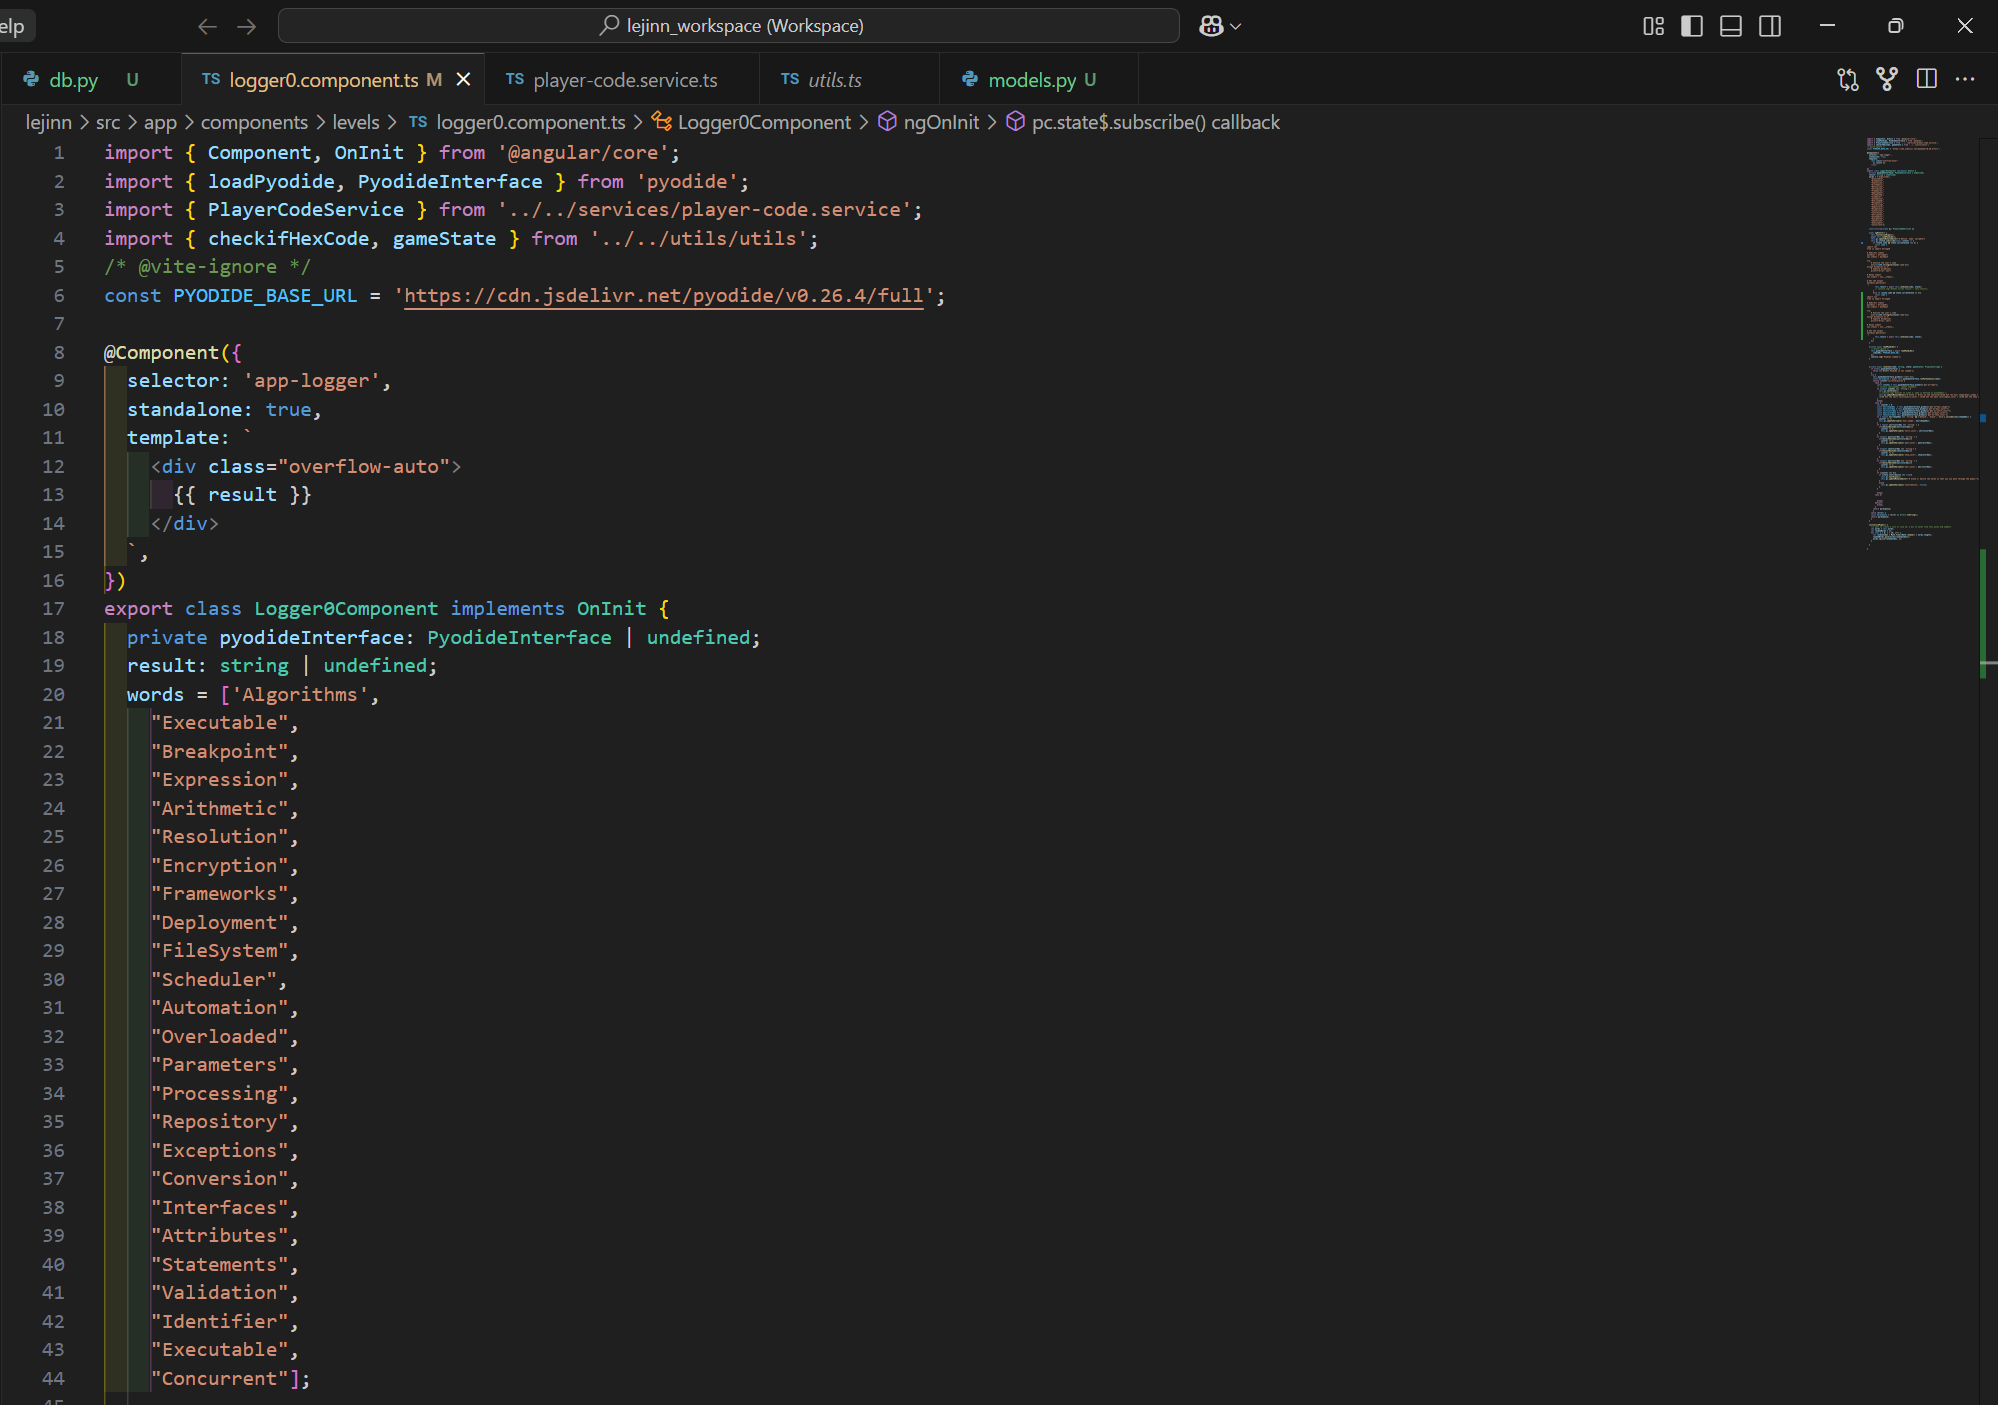
\includegraphics[width=0.3\linewidth]{images/code_editor.png}
    \caption{Code editor of IDE, a significant improvement over a basic textbox}
\end{figure}
Upon code submission, there is a reaction of the code that ran. This reaction of running code is usually known as standard output(stdout). This has to be printed out, including all results and any errors of the code. Other than just text printing with results of code submission, storytelling can take place here that is reactive upon successful results. 
